
%
\section{Theory}

% Info
% Resonnaances
% http://resonaances.blogspot.com/2011/04/update-on-forward-backward-asymmetry.html

% CDF
% http://arxiv.org/abs/1101.0034

% D0
% 10.1103/PhysRevD.84.112005

% References:
% Top FB Assymetry and Same Sign Production
% http://arxiv.org/abs/1109.3202

% http://xxx.lanl.gov/abs/arXiv:1102.3374

Recent experimental results have found statistically significant deviations from standard model predictions in events involving top quarks.
These deviations suggest that new physical models may play a role in the top sector that is experimentally testable at the LHC.

The most promising amoung these results is the measurement of an excess in forward-backward asymmetry in top quark pair production events by both the CDF and D0 experiments.
These experiments both operate on the Tevatron, which is a circular $p-\overbar{p}$ collider with a center-of-mass-energy of 1.8 TeV located at Fermilab outide of Chicaco, Illinois.

The initial directions of the proton and anti-proton beams can be used to define forward and backward directions, which are separated by a plane perpendicular to the beam line and going through the beam spot.

To lowest order, the pair production of top quarks is symmetric under interchange of the forward and backward regions.
At tree level in QCD, one does not expect an angular asymmetry in the pair production of top quarks.

However, at higher order, the Standard Model predicts a small forward-backward angular asymmetry that arises from QCD loop corrections.

\begin{figure}
  \begin{center}
    % CDF Paper: http://arxiv.org/abs/1101.0034
    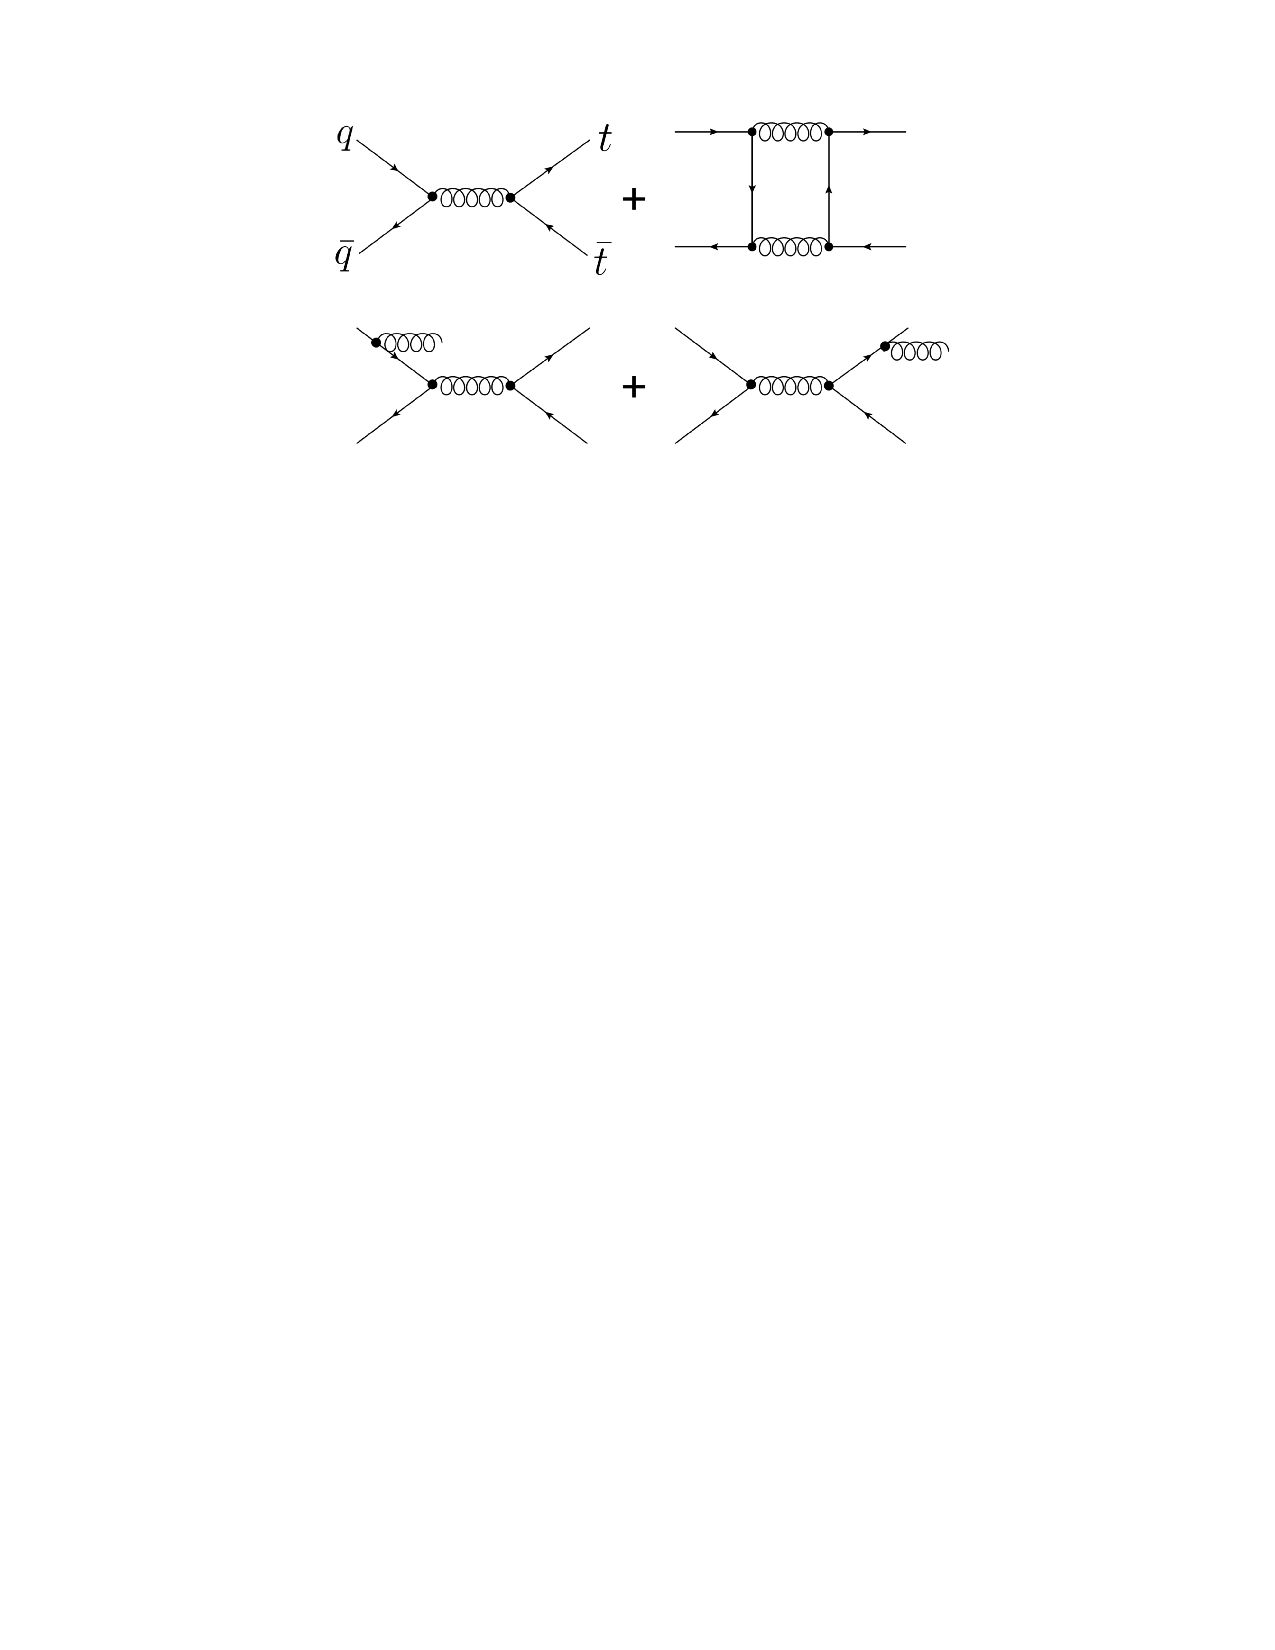
\includegraphics[width=125mm]{figures/theory/ttbarForwardBackwardFeynman}
  \end{center}
  \caption{Feynman diagrams for the pair production of $\ttbar$ in $q-\overbar{q}$ collisions.  Asymmetry in the forward-background distribution of the $\ttbar$ system arises from interference bewteen tree-level diagrams and higher-order box diagrams, as seen above.}
  \label{img:ForwardBackwardFeynman}
\end{figure}

This asymmetry can be observed experimentally using an variable that measures the directions of the top quark pairs produced at the tevatron.
Defining the difference in rapidity between the top and anti-top quarks produced to be $\Delta y = y_{t} - y_{\tbart}$, one can mesure the number of events with $\Delta y>0$ and $\Delta y<0$, which we referr to as $N(\Delta y>0)$ and $N(\Delta y < 0)$, respectively.
Using these definitions, one constructs the total $\tbart$ frame asymmetry as
\begin{equation}
  A^{\tbart} = frac{N(\Delta y>0) - N(\Delta y>0)}{N(\Delta y>0) + N(\Delta y>0)}
\end{equation}

The standard model prediction for $A^{\tbart}$ is on the order of $0.06 \pm 0.01$.%http://arxiv.org/pdf/1101.0034v1.pdf
% [1] L. G. Almeida, G. F. Sterman and W. Vogelsang, Phys. Rev. D 78, 014008 (2008).
% [2] O. Antunano, J. H. Kuhn, and G. V. Rodrigo, Phys. Rev. D 77, 014003 (2008).
% [3] M. T. Bowen, S. D. Ellis, and D. Rainwater, Phys. Rev. D 73, 014008 (2006).

Both CDF and D0 measured this variable using $\ttbar$ events where one top quark decays leptonically and the other hadronically (the single-lepton decay channel).
The presence of the charged final-state lepton can be used to differentiate the top quark from the anti-top quark's decay products.
The selection of hadronic decays on the other quark results in a higher branching ratio than a selection requiring a dileptonically decaying $\ttbar$ system.


% CDF Subsection
\subsection{CDF}

The CDF collaboration tagged $\ttbar$ events using the following event selection:
\begin{itemize}
  \item 1 selected lepton with $E_T \ge 20$ GeV and $| \eta | <$ 1
  \item 4 hadronic jets with $E_T  > 20$ GeV and $| \eta | <$ 2
  \item $\met$ > 20 GeV
\end{itemize}

The choice of jets to associate with the hadronically decaying top was made using a $\Chi^2$ kinematic fit to the full $\ttbar$ system using the mass of the W-bosons and top quarks as constraints and assigning b-tagged jets, if any, to b quarks at the parton level.
Expected signal and background distributions were evaluated using PYTHIA Monte-Carlo simulation.

The CDF measurement found a forward-backward asymmetry of $A = 0.150 \pm 0.055$ (stat+sys), which is two standard deviations away from the predicted value from NLO simulations.
In addition, the significance of this deviation was examined as a function of both the difference in rapidity ($Y$) and the invariant mass of the $\ttbar$ system:

% From Here: http://arxiv.org/pdf/1101.0034v1.pdf
% Page 13: http://arxiv.org/abs/1101.0034
\begin{tabular}{lcc}
Selection                         &   CDF Result    & SM Prediction \\
A^{\tbart}_{FB}( \Delta Y < 1.0)  & 0.026 \pm 0.118 & 0.039 \pm 0.006 \\
A^{\tbart}_{FB}( \Delta Y > 1.0)  & 0.611 \pm 0.256 & 0.123 \pm 0.008 \\
\hline
A^{\tbart}_{FB}( M_{\ttbar} < 450 GeV)   & -0.116 \pm 0.153 & 0.040 \pm 0.006 \\
A^{\tbart}_{FB}( M_{\ttbar} \ge 450 GeV) & 0.475 \pm 0.114  & 0.088 \pm 0.013 \\
\end{tabular}

Of note is the fact that the deviance of the asymmetry from prediction is a function of the invariant mass of the $\ttbar$ system.

\begin{figure}
  \begin{center}
    % CDF Paper: http://arxiv.org/abs/1101.0034
    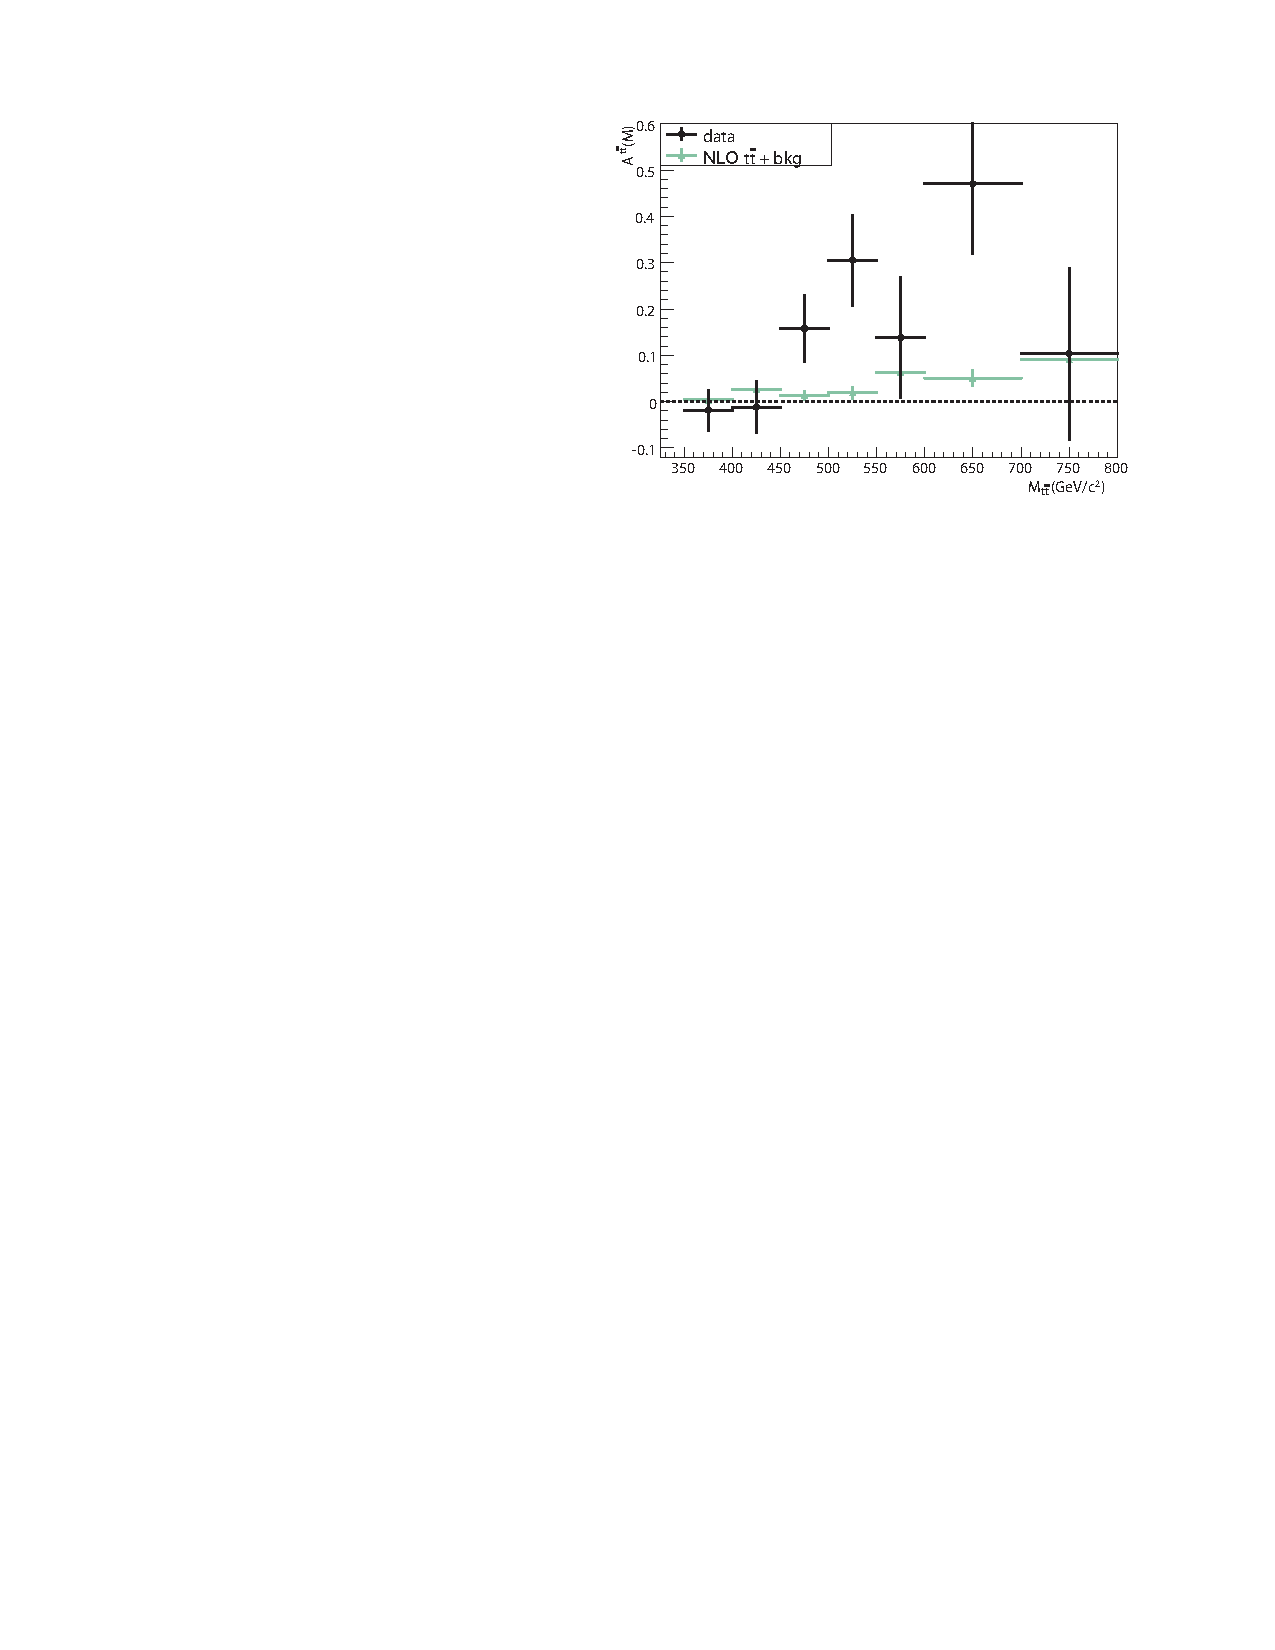
\includegraphics[width=125mm]{figures/theory/CDFAsymmetryMass}
  \end{center}
  \caption{Graph of the forward-backward asymmetry as a function of the invariant mass of the $\ttbar$ system.}
  \label{img:CDFAsymmetryMass}
\end{figure}


% D0 Subsection
\subsection{D0}

The D0 experiment selected $\ttbar$ events by triggering on either a lepton or a lepton+jet and further requiring
\begin{tabular}
  \item An isolated lepton with $p_T >$ 20 GeV and $|\eta| < $ 1.1 for electrons or $|\eta| < $ 2.0 for muons
  \item $\met >$ 20 GeV for electron events or $20 GeV < \met < 250 GeV$ for muon events
  \item $\Delta \phi(e, \met) > (2.2 - 0.045*\met / GeV)$ radians for electron events or $(p_T^\mu + \met)^2 - (p_x^\mu + \met_x)^2 - (p_y^\mu + \met_y)^2 < (250 GeV)^2$
  \item 4 jets, each with $pt > 20 GeV$ and $|\eta < 2.5|$ where the leading jet has $p_t > 40 GeV$
\end{tabular}



D0 measured an overall forward-backward asymmetry of $(9.2 \pm 3.7)%$, where the predicted value is $(2.4 \pm 0.7)%$.

\begin{tabular}{lcc}
Selection                         &   CDF Result    & SM Prediction \\
A^{\tbart}_{FB}( \Delta Y < 1.0)  6.1 \pm 4.1 & 1.4 \pm 0.6 \\
A^{\tbart}_{FB}( \Delta Y > 1.0)  21.3 \pm 9.7 & 6.3 \pm 1.6 \\
\hline
A^{\tbart}_{FB}( M_{\ttbar} < 450 GeV) & 7.8 \pm 4.8 & 1.3 \pm 0.6 \\   
A^{\tbart}_{FB}( M_{\ttbar} \ge 450 GeV) & 11.5 \pm 6.0 & 4.3 \pm 1.3 \\
\end{tabular}

The event selection used by CDF requres a selected lepton, four quarks arising from the decays of the top quarks (including on hadronic decay) and the presence of $\met$, which arises from a neutrino escaping detection.

Both D0 and CDF found 


CDF : 20.1 \pm 6.7 
D0 : 19.6 \pm 6.5 % D0 http://arxiv.org/abs/1107.4995

blah
